\documentclass{article}
% if you need to pass options to natbib, use, e.g.:
%     \PassOptionsToPackage{numbers, compress}{natbib}
% before loading neurips_2020

% ready for submission
% \usepackage{neurips_2020}

% to compile a preprint version, e.g., for submission to arXiv, add add the
% [preprint] option:
%     \usepackage[preprint]{neurips_2020}

% to compile a camera-ready version, add the [final] option, e.g.:
%     \usepackage[final]{neurips_2020}

% to avoid loading the natbib package, add option nonatbib:
\usepackage[preprint]{neurips_2020}
\usepackage[utf8]{inputenc} % allow utf-8 input
\usepackage[T1]{fontenc}    % use 8-bit T1 fonts
\usepackage{hyperref}       % hyperlinks
\usepackage{url}            % simple URL typesetting
\usepackage{booktabs}       % professional-quality tables
\usepackage{amsfonts}       % blackboard math symbols
\usepackage{nicefrac}       % compact symbols for 1/2, etc.
\usepackage{microtype}      % microtypography
\usepackage{multicol}
\usepackage{multirow}
\usepackage{diagbox}
\usepackage{subfigure}
\usepackage{tabularx}
\usepackage{graphicx}
\usepackage{indentfirst}
\usepackage{amsmath}
\setlength{\parindent}{2em}

\title{Principles of Data Science Project 1\\
        Dimension Reduction}

% The \author macro works with any number of authors. There are two commands
% used to separate the names and addresses of multiple authors: \And and \AND.
%
% Using \And between authors leaves it to LaTeX to determine where to break the
% lines. Using \AND forces a line break at that point. So, if LaTeX puts 3 of 4
% authors names on the first line, and the last on the second line, try using
% \AND instead of \And before the third author name.

\author{
  Hongzhou Liu \\
  517030910214 \\
  \texttt{deanlhz@sjtu.edu.cn} \\
  \And
  Xuanrui Hong \\
  517030910227 \\
  \texttt{hongxuanrui.1999@sjtu.edu.cn} \\
  \And
  Qilin Chen \\
  517030910155 \\
  \texttt{1017856853@sjtu.edu.cn} \\
}

\newcommand{\fix}{\marginpar{FIX}}
\newcommand{\new}{\marginpar{NEW}}

\begin{document}
\bibliographystyle{unsrt}

\maketitle

TODO:
\begin{itemize}
	\item Rewrite Feature Selection part
	\item Read and check
\end{itemize}

\begin{abstract}
\indent Datasets in real world often consist of noisies. Those noisies bring some difficulties and complexities to machine learning tasks. It is significant for us to eliminate those noisies, which leads to the topic of this project.
In this project, we conduct experiment on different dimension reduction methods, including select-k-best, variance threshold, tree-based selcetion, PCA, LDA, AutoEncoder, t-SNE and LLE.
We will observe performances of SVM on those dimension-reducted data and compare the difference among those methods. Also, we will find the optimal dimensions of each method and the optimal dimension reduction method.
\end{abstract}

\section{Method}
\subsection{Feature Selection}
\subsubsection{Select-k-best}
\indent Select-K-Best is one of the methods of univariate feature selection, which works by selecting the best features based on univariate statistical tests. It removes all but the $k$ highest scoring features. One of the parameters required for Select-K-Best is the scoring function, which mainly includes the following two:
\begin{itemize}
	\item chi2: Calculate the chi-square value of each feature, and the greater the chi-square value means the higher the correlation with the classification.
	
	\item f-classif: Calculate the F value of each feature. When the variance between the groups is much larger than the variance between the groups, that is, the gap between the groups is larger, the larger the F value.	
\end{itemize}
\subsubsection{Variance Threshold}
\indent VarianceThreshold is a simple approach to feature selection. It removes all features whose variance doesn’t meet some threshold. The principle is that features with small variance often contain less data information.
\subsubsection{Tree-based Selection}
\indent Tree-based feature selection combines SelectFromModel and ExtraTreesClassifier. SelectFromModel is a meta-transformer that can be used along with any estimator that has a $coef\_$ or $feature\_importances\_$ attribute after fitting. The features whose $coef\_$ or $feature\_importances\_$ values are below the provided threshold parameterare are considered unimportant and removed. ExtraTreesClassifier can be used to compute feature importances, which happens to cooperate with SelectFromModel to discard irrelevant features.\par
\indent In ExtraTreesClassifier, randomness is further calculated separately. Like random forest, a random subset of candidate features is used, but instead of finding the optimal discriminant attribute, a threshold is randomly selected for each candidate feature, and the best value of the randomly generated threshold is used as the segmentation principle. This usually reduces the variance of the model more, sacrifices the bias, and increases the bias. After constructing the tree, the relative rank (i.e. depth) of the features of the decision nodes in the tree can be used to evaluate the relative importance of the feature's predictability relative to the target variable. The features at the top of the tree contribute a larger score to the final prediction decision. Therefore, the predicted scores of the samples they contributed can be used as an assessment of the relative importance of features

\subsection{Feature Projection}
\subsubsection{PCA}
\indent Principal component analysis is one of the most widely used data dimensionality reduction algorithms. It performs a linear mapping of the data to a lower-dimensional space in such a way that the variance of the data in the low-dimensional representation is maximized\cite{pearson1901liii}.
Formally, the optimization goal is
\begin{eqnarray}
\centering
\max_v \frac{1}{n}\sum_{i=1}^{n}(v^Tx_i)^2=\frac{1}{n}v^TXX^Tv
\end{eqnarray}
where $v$ is the new axis.
\begin{eqnarray}
s.t.\quad v^Tv=1
\end{eqnarray}
Using Lagrange Multiplier we can get
\begin{eqnarray}
XX^Tv=\lambda v
\end{eqnarray}
We can see that $v$ is the eigenvector of $XX^T$, and $\lambda$ is the corresponding eigenvalue. Therefore, $v$ can be calculated by performing eigenvalue decomposition to the co-variance matrix $XX^T$. Then we can get the data after dimensionality reduction.
\subsubsection{Kernel PCA}
\indent In general, principal components analysis is suitable for linear dimensionality reduction of data. Kernel PCA can achieve nonlinear dimensionality reduction of data and is used to process linear inseparable data sets.\\
\indent The general idea of Kernel PCA is: for the matrix in the input space, we first use a non-linear mapping to map all samples in a high-dimensional or even infinite-dimensional space, and then perform PCA dimensionality reduction in this high-dimensional space.
So Kernel PCA will replace $X$ in PCA by $\phi(X)$ to do this mapping, and $\phi(X)$ is called kernel. However, $\phi(X)$ may not have an explicit form, sometimes it will map $X$ into a infinite dimension space. The kernel trick solves this problem by directly compute the inner product between $\phi(X)$ and $\phi(Y)$ by
\begin{eqnarray}
\centering
K(X, Y) = \phi(X)^{T}\phi(Y)
\end{eqnarray}
So, using Lagrange Multiplier we will instead get
\begin{eqnarray}
\centering
K(X, X)v=\lambda v
\end{eqnarray}
There're different kinds of kernels
\begin{itemize}
	\item Linear Kernel: $K(\boldsymbol{x}, \boldsymbol{y})=\boldsymbol{x}^{T}\boldsymbol{y}$
	\item Polynomial Kernel: $K(\boldsymbol{x}, \boldsymbol{y})=(\boldsymbol{x}^{T}\boldsymbol{y}+c)^d$
	\item Gaussian Kernel (RBF Kernel): $K(\boldsymbol{x},\boldsymbol{y})=\exp(-\dfrac{\left\| \boldsymbol{x}-\boldsymbol{y}\right\|^2}{2\sigma^2})$
	\item Sigmoid Kernel: $K(\boldsymbol{x},\boldsymbol{y})=\tanh(\alpha \boldsymbol{x}^{T}\boldsymbol{y}+c)$
\end{itemize}
\subsubsection{LDA}
\indent Linear discriminate analysis is commonly used as dimensionality reduction technique. Its main idea is to project the samples on a straight line so that the projections of similar samples are as close as possible, and the projection points of heterogeneous samples are as far as possible. 
	\begin{figure}[htbp]
		\centering
		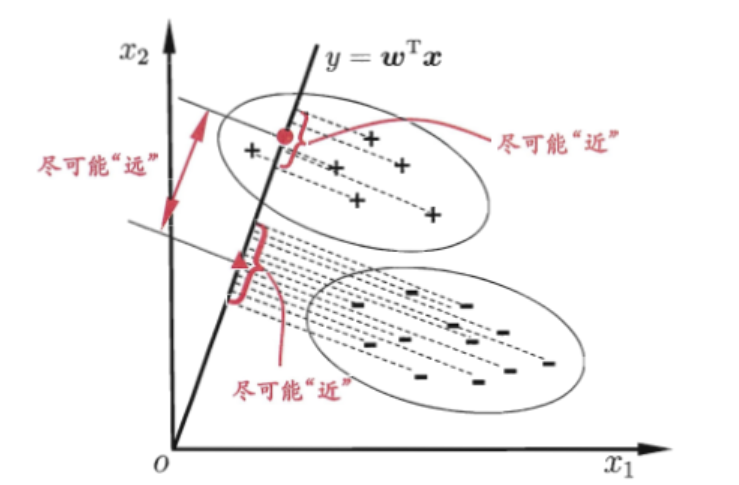
\includegraphics[scale=0.3]{figure/LDA.png}
		\caption{Two-dimensional illustration of LDA.}
		\label{fig:LDA}
	\end{figure}\cite{zhihuazhou2016ml}\par
\indent The key step of LDA:
\begin{itemize}
		\item Standardize d-dimensional data (d is the number of features).
		
		\item For each category, calculate the d-dimensional mean vector.
		
		\item Construct inter-class scatter matrix $S_B$ and intra-class scatter matrix $S_W$.
		
		\item Calculate the eigenvalues and corresponding eigenvectors of the matrix $S^{-1}_WS_B$.
		
		\item Select the eigenvectors corresponding to the first $k$ eigenvalues to construct a $d \times k$ dimension transformation matrix $W$, where the eigenvectors are arranged in columns.
		
		\item Use the transformation matrix $W$ to map the samples to the new feature subspace.
		
\end{itemize}
\subsubsection{AutoEncoder}
\indent An autoencoder is a type of artificial neural network used to learn efficient data codings in an unsupervised manner.\cite{kramer1991nonlinear}The purpose of autoencoder is to train a neural network for sample dimensionality reduction, and the sample after dimensionality reduction can reconstruct the original sampel well. \par
\indent It contains encoder and decoder. The coding network belongs to the dimension reduction part, and the role is to reduce the high-dimensional original data to a low-dimensional nested structure with a certain number of dimensions; the decoding network belongs to the reconstruction part, which can be regarded as the reverse process of the coding network. There is also an intersection between the encoding network and the decoding network, called the "code layer", which is the core of the entire self-encoding network  and can determine the essential dimensions of high-dimensional datasets.
\begin{figure}[htbp]
	\centering
	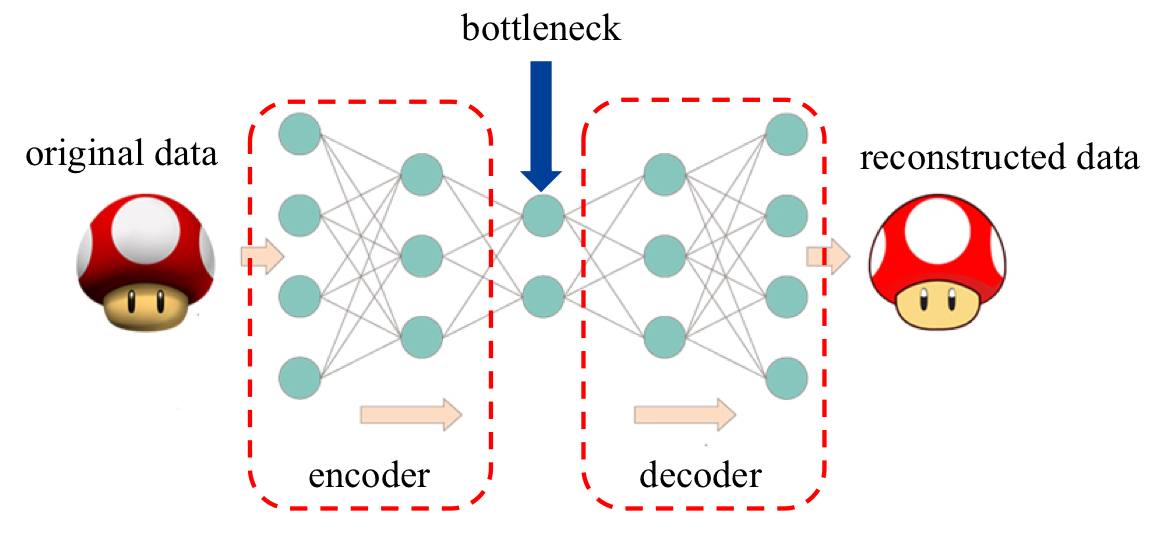
\includegraphics[scale=0.2]{figure/Autoencoder.jpg}
	\caption{Autoencoder.}
	\label{fig:autoencoder}
\end{figure}\par
\subsection{Feature Learning}
\subsubsection{t-SNE}
\indent T-distributed stochastic neighbor embedding is a machine learning algorithm for dimensionality reduction, proposed by Laurens van der Maaten and Geoffrey Hinton in 2008.\cite{maaten2008visualizing}It is a nonlinear dimensionality reduction technique. T-SNE obtains $\tilde{x}$ from $x$ and maintains the relative distance as much as possible. Its main steps are:
\begin{itemize}
	\item  Evaluate the similarity of data point $x_i$ and data point $x_j$ by
	\begin{eqnarray}
	p_{j|i}=\frac{(1+\Vert x_i-x_j \Vert^2)^-1}{\sum_{k\neq i}(1+\Vert x_i-x_k \Vert^2)^-1}
	\end{eqnarray}
	
	\item  Meature similarity of data point $\tilde{x_i}$ and data point $\tilde{x_j}$ by
	\begin{eqnarray}
	q_{j|i}=\frac{(1+\Vert \tilde{x_i}-\tilde{x_j} \Vert^2)^-1}{\sum_{k\neq i}(1+\Vert \tilde{x_i}-\tilde{x_k} \Vert^2)^-1}
	\end{eqnarray}
	
	\item  Minimize the $Kullback-Leibler divergence$ of the distribution $Q$ from the distribution $P$, that is
	\begin{eqnarray}
	L = \sum_{i}KL(P_i\Vert Q_i)=\sum_{i}\sum_{j}p(i|j)log\frac{p_{j|i}}{q_{j|i}}
	\end{eqnarray}
\end{itemize}

\indent Besides, t-SNE is the deformation of SNE. The difference is that t-SNE uses t-distribution while SNE uses Gaussian distribution.
\begin{figure}[htbp]
	\centering
	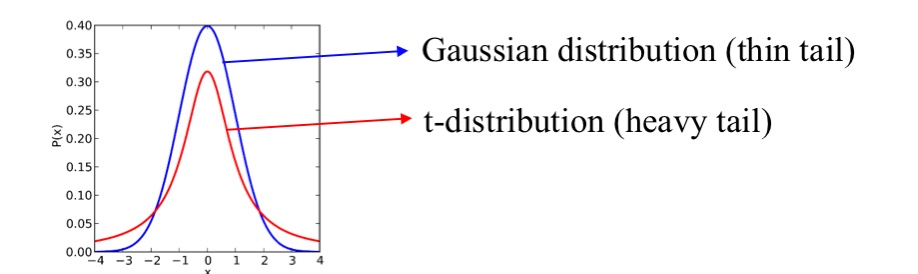
\includegraphics[scale=0.3]{figure/SNE.jpg}
	\caption{t-SNE and SNE.}
	\label{fig:SNE}
\end{figure}\par

\subsubsection{LLE}
Locally Linear Embedding (LLE) is a member of the manifold learning algorithm and is a nonlinear dimensionality reduction method. LLE was invented in 2000 and published in the journal Sience.\cite{roweis2000nonlinear}LLE algorithm tries to maintain the linear relationship between samples in the neighborhood. As shown in \ref{fig:LLE}, the sample $x_i$ in the high-dimensional space can be reconstructed from its neighbor sample $x_j,x_k,x_l$ through linear combination, i.e.
\begin{eqnarray}
x_i = w_{ij}x_j+w_{ik}x_k+x_{il}x_l
\end{eqnarray}
\begin{figure}[htbp]
	\centering
	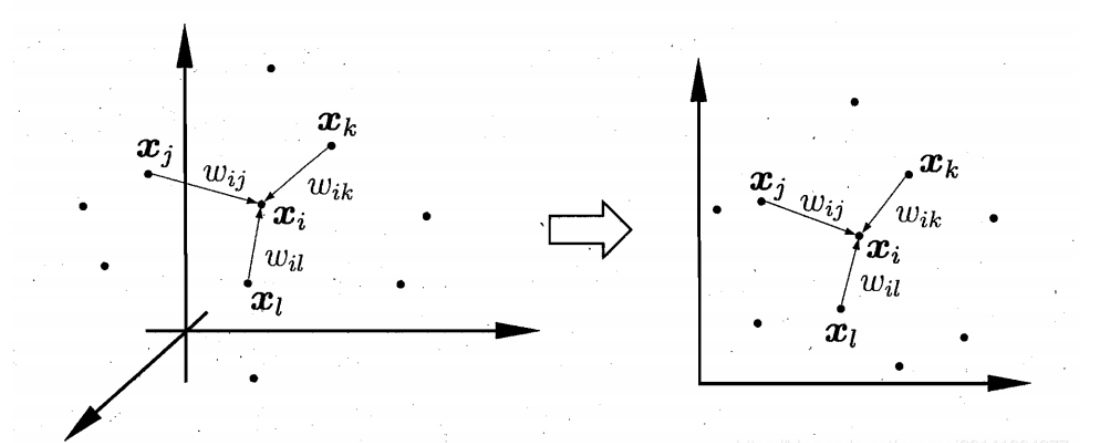
\includegraphics[scale=0.3]{figure/LLE.png}
	\caption{LLE.}
	\label{fig:LLE}
\end{figure}\par
\indent Its main steps are:
\begin{itemize}
	\item Learn the linear relation $W$ between each sample and its neighbors, which can be formalized as:
	\begin{eqnarray}
	W = \mathop{\arg\min}_{W}\sum_{i=1}^{m}\Vert x_i-\sum_{j\in N(i)}w_{ij}x_j\Vert^2 
	\end{eqnarray}
	where $N(i)$ is the k-nearest neighbors of $x_i$
	
	\item  Reconstruct the low-dimensional features:
	\begin{eqnarray}
	Z = \mathop{\arg\min}_{Z}\sum_{i=1}^{m}\Vert z_i-\sum_{j\in N(i)}w_{ij}z_j\Vert^2 
	\end{eqnarray}
	where $z_i$ is the sample after dimensionality reduction of $x_i$
\end{itemize}

\section{Experiment}
\subsection{Baseline}
\par The dataset we use is \href{https://cvml.ist.ac.at/AwA2/}{Animals with Attributes (AwA2)}, which consists of 37322 images of 50 animal classes. We will do our experiment on pre-extracted deep learning features with 2048 dimensions of AwA2.
\par We will split 60\% of the features and labels into training set and 40\% for testing set.
We feed the training set without dimension reduction into SVM and test the model on testing set. Then we observe the optimal hyper-parameter by k-fold validation. The optimal hyper-parameters of linear SVM and RBF kernel SVM on AwA2 is \ref{baseline}
\begin{table}[htbp]
	\centering
	\newcommand{\tabincell}[2]{\begin{tabular}{@{}#1@{}}#2\end{tabular}}
	\renewcommand\arraystretch{1.0}
	\caption{SVM}
	\label{baseline}%
	\begin{tabular}{c|c|c}
		\hline
			& C & Acc.(\%)\\
		\hline
		Linear & 0.002 & 93.2815\\
		\hline
		RBF Kernel & 5.0 & 93.5160\\
		\hline
\end{tabular}
\end{table}
\subsection{Feature Selection}
\subsubsection{Select-K-Best}
Select-K-Best belongs to univariate feature selection. It removes all but the $k$ highest scoring features. There are many options for the parameter $score\_func$ of this method and we chose the $f\_classif$. In this section, two experiment settings can derive from the rule: We use Select-K-Best on different number of aim component $[2, 5, 10, 20, 50, 100, 200, 500, 750, 1000, 1200, 1500, 2000]$, and we give our results on two types of kernel: linear kernel and radial basis function kernel. We adopt classifiction accuracy as metric in this section.

We summarize the experimental results of Select-K-Best in Tab. \ref{base1} and Fig. \ref{Figure1}. As is shown, linear Select-K-Best model and RBF Select-K-Best model expectively exhibit the best performances at 1000 components and 750 components, reaching 93.01\% and 92.96\% on the classification task. We can compare the result with the simple linear SVM and simple RBF SVM, find the Select-K-Best model's performance is worse than the baselines, and we deem the reason is that Select-K-Best reduces the dimension at the cost of reducing a little accuracy. Besides, more dimensions results in higher accuracy.

We give the 2-components scattering figure of different kernel and dataset in Fig. \ref{Figure2}, from which we can see that the data reduced to 2 dimensions using the Select-K-Best method are clustered together and cannot be well classified. This can also be inferred from the Tab. \ref{base1}.

\begin{table}[htbp]
	\centering
	\newcommand{\tabincell}[2]{\begin{tabular}{@{}#1@{}}#2\end{tabular}}
	\renewcommand\arraystretch{1.0}
	\caption{Comparison of Select-K-Best and baslines in Classification Task}
	\label{base1}%
	\begin{tabular}{@{}p{2.5cm}<{\centering}|c|c}
		\hline
		\multirow{2}{*}{\diagbox[height=2\line,width=2.7cm,font=\tiny,trim=lr]{$d$}{Acc.}{$\mathit{M}$}} &\multicolumn{2}{c}{Select-K-Best+SVM}\\
		\cline{2-3}
			& {Linear kernel(\%)} & {RBF kernel(\%)}\\
		\cline{2-3}
		\hline
		Baseline & 93.28 & 93.52\\
		\hline
		2   & 12.45 & 16.05\\
		\hline
		5   & 23.33 & 35.80\\
		\hline
		10  & 32.88 & 48.84\\
		\hline
		20  & 57.59 & 71.85\\
		\hline
		50  & 79.86 & 85.92\\
		\hline
		100 & 87.38 & 89.85\\
		\hline
		200 & 90.69 & 91.55\\
		\hline
		500 & 92.45 & 92.75\\
		\hline
		750 & 92.77 & \textbf{92.96}\\
		\hline
		1000 & \textbf{93.01} & 92.92\\
		\hline
		1200 & 92.88 & 92.84\\
		\hline
		1500 & 92.88 & 91.55\\
		\hline
		2000 & 92.98 & 91.96\\
		\hline
\end{tabular}
\end{table}

\begin{figure}[htbp]
	\centering
	\subfigure[metric accuracy comparison on linear Select-K-Best]{
		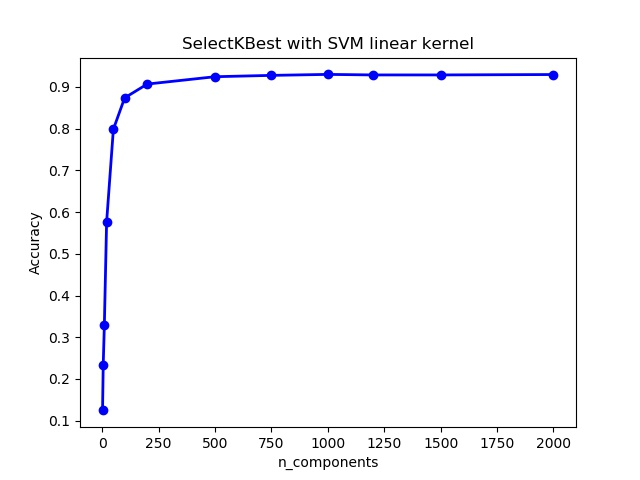
\includegraphics[width=5.5cm]{figure/SelectKBest_linear.jpg}
		%\caption{fig1}
	}
	\quad
	\subfigure[metric accuracy comparison on RBF Select-K-Best]{
		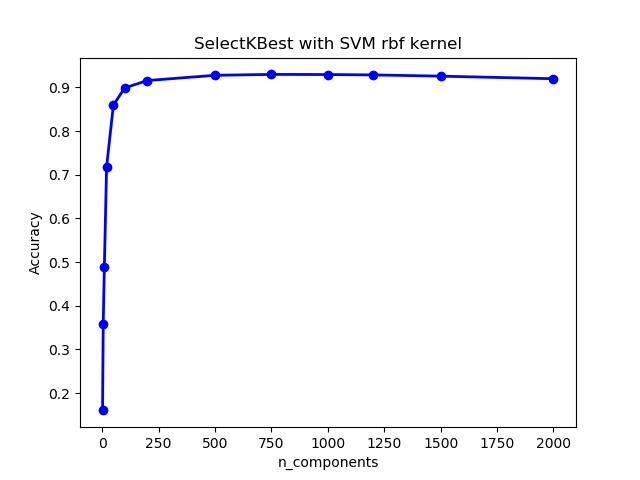
\includegraphics[width=5.5cm]{figure/SelectKBest_rbf.jpg}
	}
	\caption{Select-K-Best performance on linear kernel and RBF kernel}
	\label{Figure1}
\end{figure}

\begin{figure}[htbp]
	\centering
	\subfigure[Trainset 2D scatter with Select-K-Best]{
		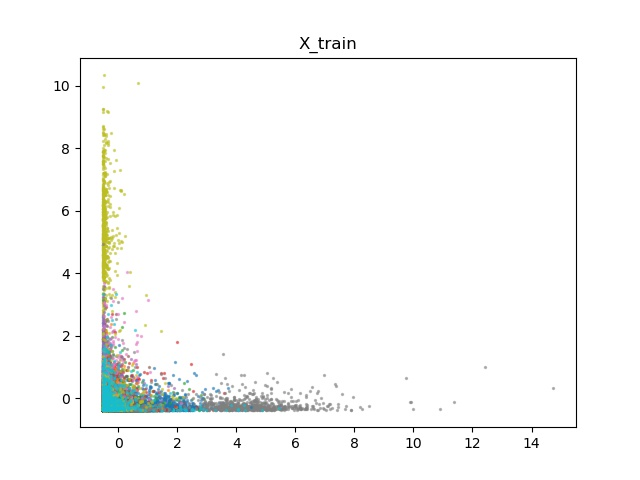
\includegraphics[width=5.5cm]{figure/X_train_scatter_2d_SelectKBest.jpg}
		%\caption{fig1}
	}
	\quad
	\subfigure[Testset 2D scatter with Select-K-Best]{
		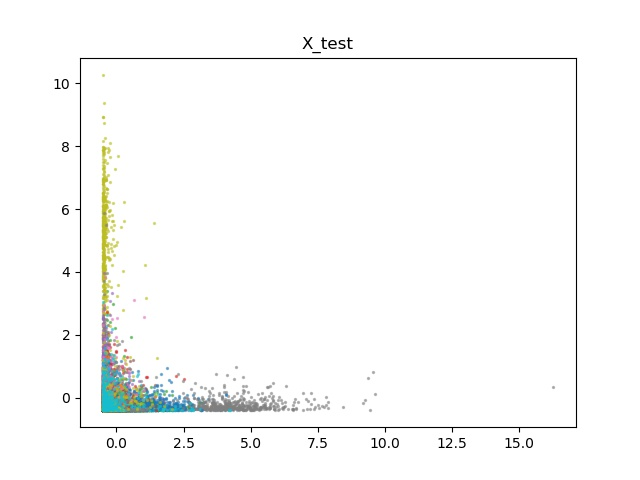
\includegraphics[width=5.5cm]{figure/X_test_scatter_2d_SelectKBest.jpg}
	}
	\caption{Dataset 2D scatter with Select-K-Best}
	\label{Figure2}
\end{figure}
\subsubsection{Variance Threshold}
VarianceThreshold is one of the simple feature selection methods, removing all features whose variance is less than the threshold. In this section, two experiment settings can derive from the rule: We use Variance Threshold on different number of aim component $[0.1, 0.2, 0.3, 0.5, 0.7, 0.9]$, and we give our results on two types of kernel: linear kernel and radial basis function kernel. We adopt classifiction accuracy as metric in this section.

We summarize the experimental results of Variance Threshold in Tab. \ref{base2} and Fig. \ref{Figure3}. As is shown, the linear Variance Threshold model and the RBF Variance Threshold model exhibit the best performance on 0.1 components and 0.3 components, with data dimensions of 1883 and 1022, and classification accuracy of 92.96\% and 93.08\% respectively. We can see that Variance Threshold is similar to Select-K-Best because their classification accuracy is not as good as baselines. It also reduces dimensionality at the cost of accuracy.


\begin{table}[htbp]
	\centering
	\newcommand{\tabincell}[2]{\begin{tabular}{@{}#1@{}}#2\end{tabular}}
	\renewcommand\arraystretch{1.0}
	\caption{Comparison of Variance Threshold and baselines in Classification Task}
	\label{base2}%
	\begin{tabular}{@{}p{2.5cm}<{\centering}|c|c|c}
		\hline
		\multirow{2}{*}{\diagbox[height=2\line,width=2.9cm,font=\tiny]{$\theta$}{Acc.}{$\mathit{M}$}} &\multicolumn{3}{c}{Variance Threshold+SVM}\\
		\cline{2-4}
		& {Dimension} & {Linear kernel(\%)} & {RBF kernel(\%)}\\
		\hline
		Baseline & 2048 & 93.28 & 93.52\\
		\hline
		0.1   & 1883 & \textbf{92.96} & 92.24\\
		\hline
		0.2   & 1345 & 92.94 & 92.75\\
		\hline
		0.3   & 1022 & 92.87 & \textbf{93.08}\\
		\hline
		0.5   & 620  & 92.94 & 92.98\\
		\hline
		0.7   & 401  & 92.63 & 92.73\\
		\hline
		0.9   & 271  & 91.88 & 92.30\\
		\hline
	\end{tabular}
\end{table}

\begin{figure}[htbp]
	\centering
	\subfigure[metric accuracy comparison on linear Variance Threshold]{
		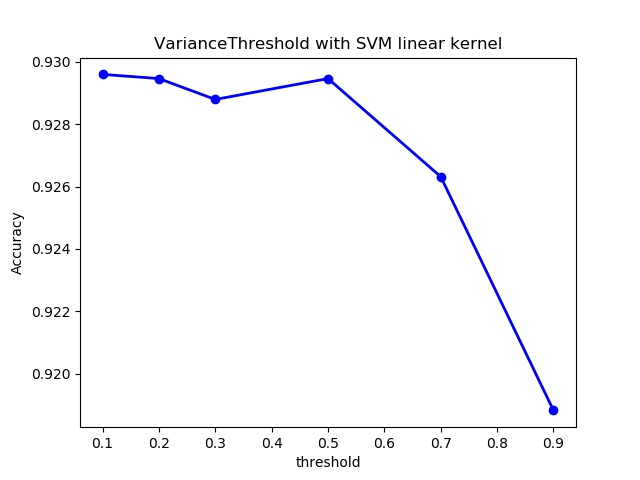
\includegraphics[width=5.5cm]{figure/VarianceThreshold_linear.jpg}
		%\caption{fig1}
	}
	\quad
	\subfigure[metric accuracy comparison on RBF Variance Threshold]{
		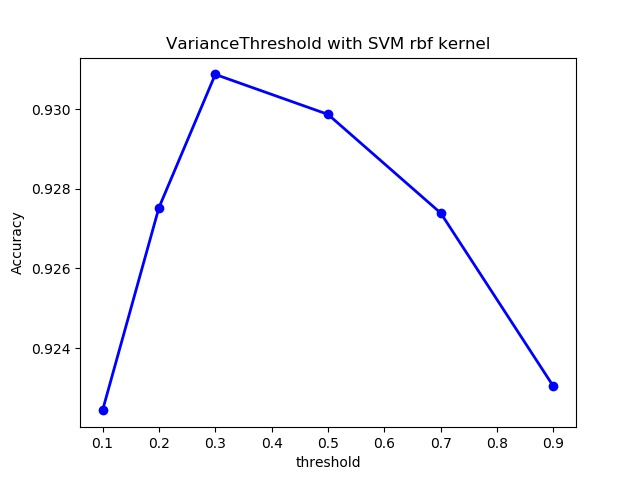
\includegraphics[width=5.5cm]{figure/VarianceThreshold_rbf.jpg}
	}
	\caption{VarianceThreshold performance on linear kernel and RBF kernel}
	\label{Figure3}
\end{figure}

\subsubsection{Tree-based Selection}
Tree-based predictive models can be used to calculate the importance of features, so they can be used to remove irrelevant features. In this section, two experiment settings can derive from the rule: We use tree-based selection on different number of aim component $[2, 4, 8, 16, 32, 64]$, and we give our results on two types of kernel: linear kernel and radial basis function kernel. We adopt classifiction accuracy as metric in this section.

We summarize the experimental results of tree-based selection in Tab. \ref{base3} and Fig. \ref{Figure4}. As is shown, the linear Variance Threshold model and the RBF Variance Threshold model exhibit the best performance both on 4 components, with data dimensions of 564, and classification accuracy of 92.63\% and 92.84\% respectively. We can see that the best classification accuracy of tree-based selection is not as good as Select-K-Best and Variance Threshold. According to the decision tree, the reason may be that for data with inconsistent sample sizes in each category, the information gain is biased towards those features with more values.


\begin{table}[htbp]
	\centering
	\newcommand{\tabincell}[2]{\begin{tabular}{@{}#1@{}}#2\end{tabular}}
	\renewcommand\arraystretch{1.0}
	\caption{Comparison of Tree-based selection and baslines in Classification Task}
	\label{base3}%
	\begin{tabular}{@{}p{2.5cm}<{\centering}|c|c|c}
		\hline
		\multirow{2}{*}{\diagbox[height=2\line,width=2.9cm,font=\tiny]{$\#est.$}{Acc.}{$\mathit{M}$}} &\multicolumn{3}{c}{Tree-based selection+SVM}\\
		\cline{2-4}
			& {Dimension} & {Linear kernel(\%)} & {RBF kernel(\%)}\\
		\hline
		Baseline & 93.28 & 93.52\\
		\hline
		2   & 523 & 92.61 & 92.69\\
		\hline
		4   & 564 & 92.63 & 92.84\\
		\hline
		8   & 563 & 92.47 & 92.80\\
		\hline
		16   & 609  & 92.59 & 92.67\\
		\hline
		32   & 609  & 92.58 & 92.81\\
		\hline
		64   & 600  & 92.59 & 92.81\\
		\hline
\end{tabular}
\end{table}

\begin{figure}[htbp]
	\centering
	\subfigure[metric accuracy comparison on linear Tree-based selection]{
		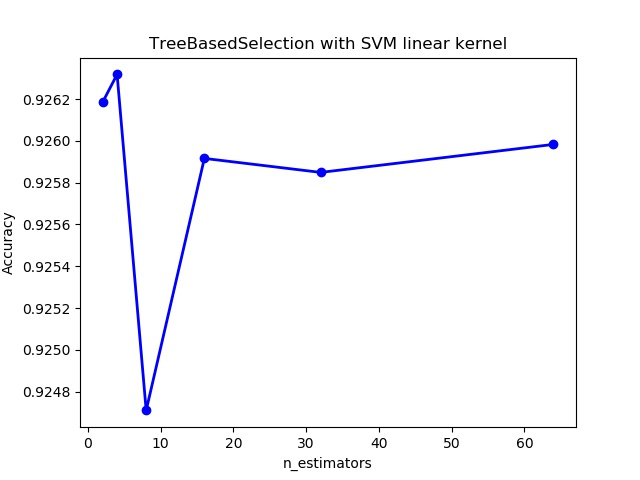
\includegraphics[width=5.5cm]{figure/TreeBasedSelection_linear.jpg}
		%\caption{fig1}
	}
	\quad
	\subfigure[metric accuracy comparison on RBF Tree-based selection]{
		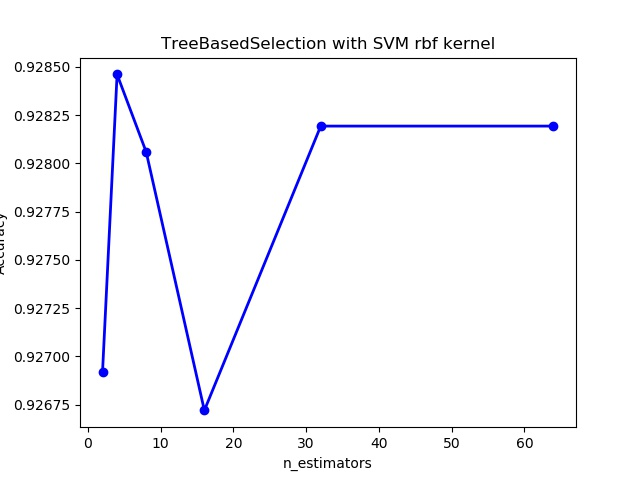
\includegraphics[width=5.5cm]{figure/TreeBasedSelection_rbf.jpg}
	}
	\caption{Tree-based selection performance on linear kernel and RBF kernel}
	\label{Figure4}
\end{figure}

\subsection{Feature Projection}
\subsubsection{PCA}
Principal component analysis (PCA) is the most typical feature projection method based on dimension reduction, since PCA provides a roadmap for how to reduce a complex data set to a lower dimension to reveal the sometimes hidden, simplified dynamics that often underlie it. Kernel principal component analysis (kernel PCA) provides an extension of traditional PCA using techniques of kernel methods, which project source data into a higher dimensional space, providing with better reduction and classification performance. In this section, two experiment settings can derive from the rule: We use kernel PCA on different number of aim component $[2, 5, 10, 20, 50, 100, 200, 500, 750, 1000, 1200, 1500, 2000]$, and we give our results on two types of kernel: linear kernel and radial basis function kernel. We adopt classifiction accuracy as metric in this section.

We summarize the experimental results of kernel PCA in Tab. \ref{baseline1} and Fig. \ref{Fig1}. As is shown, linear kernel PCA model and RBF kernel PCA model expectively exhibit the best performances at 200 components and 750 components, reaching $92.20\%$ and $92.50\%$ on the classification task. We can compare the result with the simple linear SVM and simple RBF SVM, find the kernel PCA model's performance is worse than the baselines, and we deem the reason is that compoents reduction of PCA remove some effective feature as it remove the most noisy feature. And we can find RBF kernel have better performance than linear kernel in PCA tasks and none-PCA tasks, it proves the provided dataset have some features which can't be handled merely by linear kernel. Besides, in kernel PCA tasks, we can find if we have less components, RBF kernel have better performance than linear kernel.

We give the 2-components scattering figure of different kernel and dataset in Fig. \ref{Fig2}, which can support the result that RBF kernel have better performance than linear kernel since the RBF figure can be better splited. What's more, if we compare the trainset and testset, we can find the dataset is randomly splited.

\begin{table}[htbp]
	\centering
	\newcommand{\tabincell}[2]{\begin{tabular}{@{}#1@{}}#2\end{tabular}}
	\renewcommand\arraystretch{1.0}
	\caption{Comparison of kernel PCA and baslines in Classification Task}
	\label{baseline1}%
	\begin{tabular}{@{}p{2.5cm}<{\centering}|c|c}
		\hline
		\multirow{2}{*}{\diagbox[height=2\line,width=2.9cm,font=\tiny]{$d$}{Acc.}{$\mathit{M}$}} &\multicolumn{2}{c}{PCA+SVM}\\
		\cline{2-3}
			& {Linear kernel(\%)} & {RBF kernel(\%)}\\
		\cline{2-3}
		\hline
		Baseline & 93.28 & 93.52\\
		\hline
		2   & 12.46 & 19.68\\
		\hline
		5   & 40.31 & 59.68\\
		\hline
		10   & 68.99 & 78.25\\
		\hline
		20   & 82.27 & 87.07\\
		\hline
		50  & 89.31 & 90.53\\
		\hline
		100  & 91.37 & 91.66\\
		\hline
		200  & \textbf{92.20} & 91.94\\
		\hline
		500  & 92.14 & 92.42\\
		\hline
		750  & 91.90 & \textbf{92.50}\\
		\hline
		1000  & 91.70 & 92.44\\
		\hline
		1200  & 91.78 & 92.26\\
		\hline
		1500  & 91.57 & 91.85\\
		\hline
		2000  & 91.64 & 88.08\\
		\hline
	\end{tabular}
\end{table}

\begin{figure}[htbp]
\centering
\subfigure[metric accuracy comparison on linear PCA]{
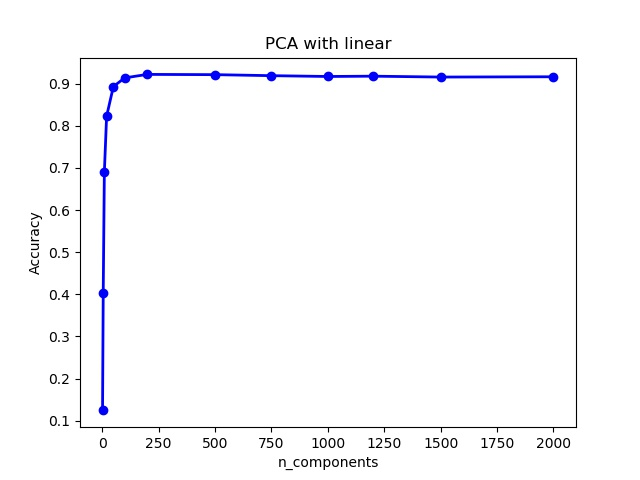
\includegraphics[width=5.5cm]{figure/PCA_linear.jpg}
%\caption{fig1}
}
\quad
\subfigure[metric accuracy comparison on RBF PCA]{
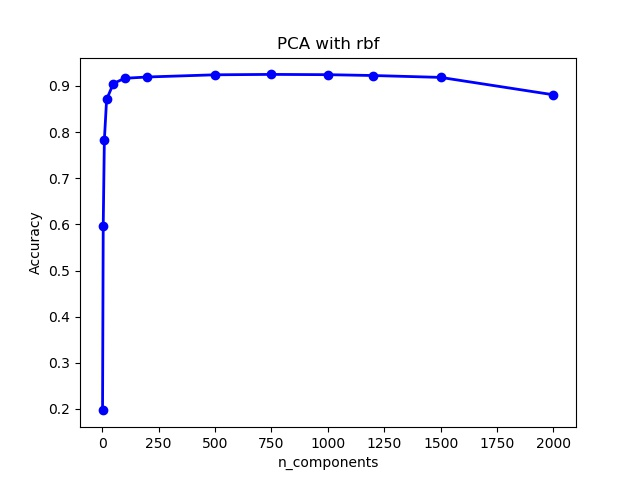
\includegraphics[width=5.5cm]{figure/PCA_rbf.jpg}
}
\caption{Kernel PCA performance on linear kernel and RBF kernel}
\label{Fig1}
\end{figure}

\begin{figure}[htbp]
\centering
\subfigure[Trainset 2D scatter with linear PCA]{
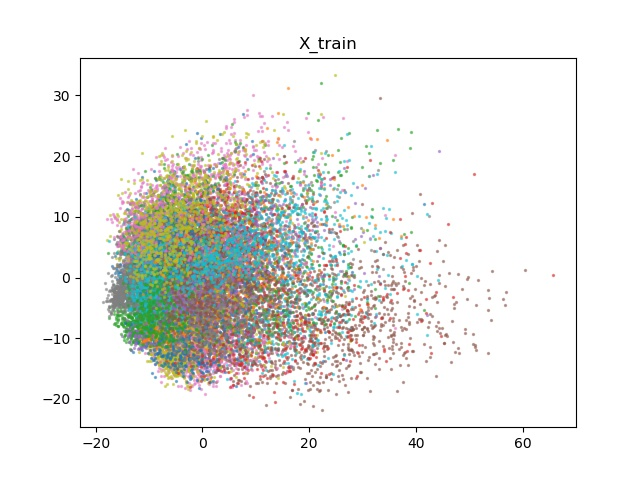
\includegraphics[width=5.5cm]{figure/X_train_scatter_2d_linear.jpg}
%\caption{fig1}
}
\quad
\subfigure[Testset 2D scatter with linear PCA]{
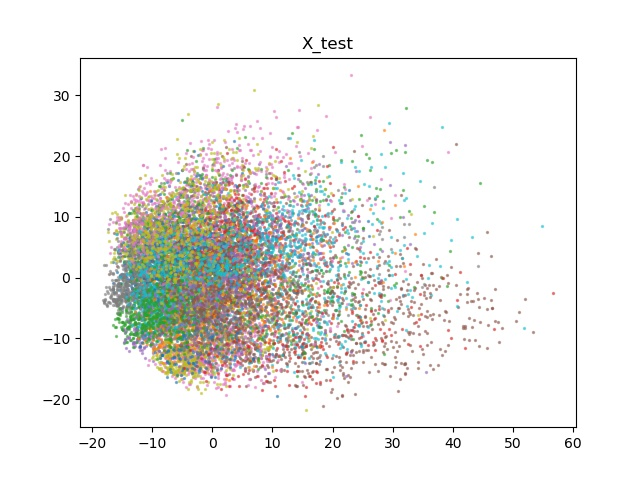
\includegraphics[width=5.5cm]{figure/X_test_scatter_2d_linear.jpg}
}
\quad
\subfigure[Trainset 2D scatter with RBF PCA]{
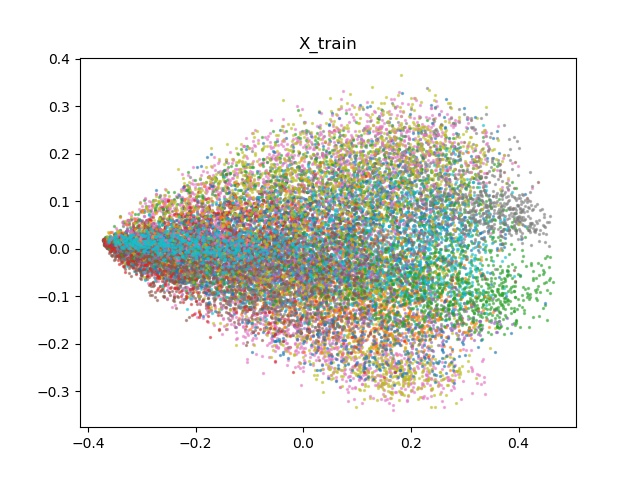
\includegraphics[width=5.5cm]{figure/X_train_scatter_2d_rbf.jpg}
}
\quad
\subfigure[Testset 2D scatter with RBF PCA]{
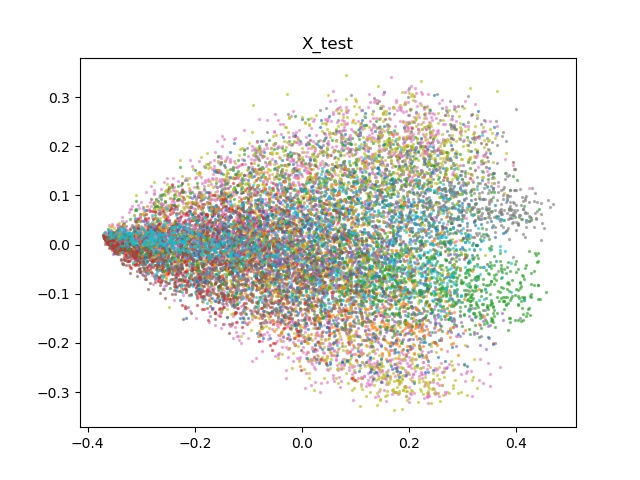
\includegraphics[width=5.5cm]{figure/X_test_scatter_2d_rbf.jpg}
}
\caption{Dataset 2D scatter with linear kernel and RBF kernel}
\label{Fig2}
\end{figure}

\subsubsection{LDA}

Linear discriminate analysis (LDA) is a dimension reduction technique that is closely related to principal component analysis (PCA) and factor analysis in that they both look for linear combinations of variables which best explain the data. However, in contrast, LDA explicitly attempts to model the difference between the classes of data. In this section, we use LDA model to project features into [2, 3, 5, 10, 20, 30, 40] components and respectively combine RBF SVM and Linear SVM to finish the classification task. We adopt classifiction accuracy as metric in this section.

We summarize the experimental results of LDA-based model in Tab. \ref{baseline2} and Fig. \ref{Fig3}. As is shown, based on LDA method, Linear kernel SVM and RBF kernel SVM have better performance as the compoents number increase and reach accuracy of $90.56\%$ and $91.47\%$ respectively. As PCA-based method, some components loss may occur while we reduce the data dimension, but with the components number increase, we can find the accuracy nearly closed to the traditional SVM model. Besides, we can find RBF kernel have better performance than linear kernel in LDA tasks and none-LDA tasks, it proves the provided dataset have some features which can't be handled merely by linear kernel. Especially, in LDA tasks, we can find if we have less components, RBF kernel have much better performance than linear kernel.

We give the 2-components scattering figure of different kernel and dataset in Fig. \ref{Fig4}. Compared with Fig. \ref{Fig2}, we can conclude LDA have better classes distance than PCA, which supports the correctness of the experiment. And we can find the random splitness of the dataset is covered.

\begin{table}[htbp]
	\centering
	\newcommand{\tabincell}[2]{\begin{tabular}{@{}#1@{}}#2\end{tabular}}
	\renewcommand\arraystretch{1.0}
	\caption{Comparison of LDA-based SVM and baslines in Classification Task}
	\label{baseline2}%
	\begin{tabular}{@{}p{2.5cm}<{\centering}|c|c}
		\hline
		\multirow{2}{*}{\diagbox[height=2\line,width=2.9cm,font=\tiny]{$d$}{Acc.}{$\mathit{M}$}} &\multicolumn{2}{c}{LDA+SVM}\\
		\cline{2-3}
			& {Linear kernel(\%)} & {RBF kernel(\%)}\\
		\cline{2-3}
		\hline
		Baseline & 93.28 & 93.52\\
		\hline
		2   & 16.02 & 30.39\\
		\hline
		3   & 19.63 & 39.80\\
		\hline
		5   & 38.93 & 57.69\\
		\hline
		10   & 58.08 & 71.36\\
		\hline
		20   & 77.61 & 82.75\\
		\hline
		30   & 87.80 & 89.75\\
		\hline
		40   & \textbf{90.56} & \textbf{91.47}\\
		\hline
	\end{tabular}
\end{table}

\begin{center}
\begin{figure}[htbp]
\centering
\subfigure[metric accuracy comparison on LDA with linear SVM]{
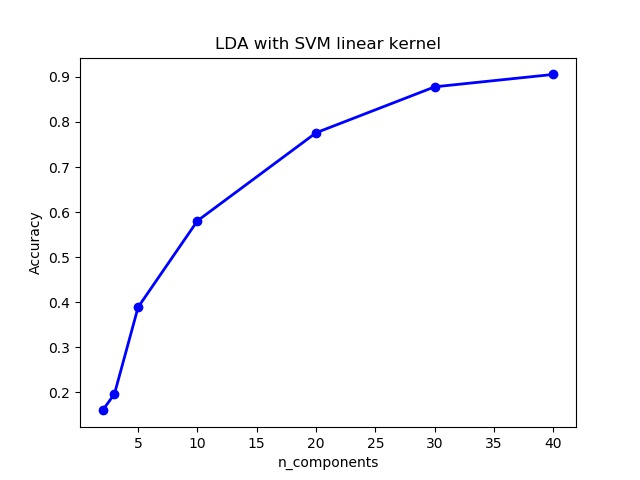
\includegraphics[width=5.5cm]{figure/LDA_linear.jpg}
%\caption{fig1}
}
\quad
\subfigure[metric accuracy comparison on LDA with RBF SVM]{
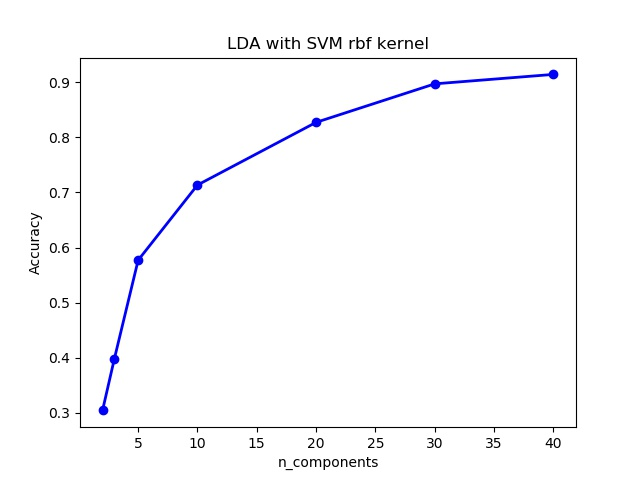
\includegraphics[width=5.5cm]{figure/LDA_rbf.jpg}
}
\caption{LDA-based model performance on linear kernel SVM and RBF kernel SVM}
\label{Fig3}
\end{figure}
\end{center}

\begin{center}
\begin{figure}[htbp]
\centering
\subfigure[Trainset 2D scatter with LDA]{
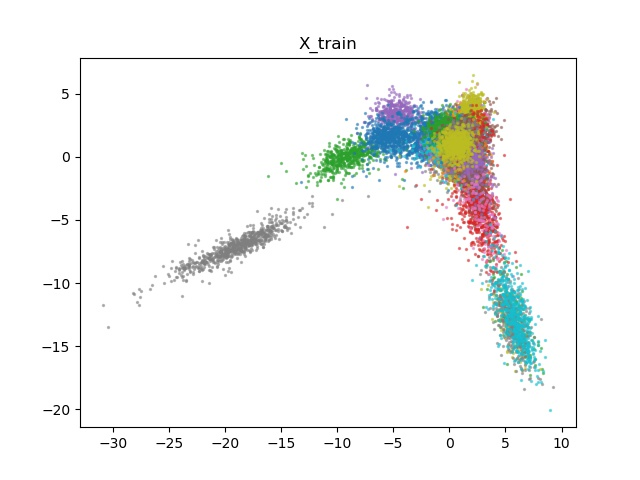
\includegraphics[width=5.5cm]{figure/X_train_scatter_2d_LDA.jpg}
%\caption{fig1}
}
\quad
\subfigure[Testset 2D scatter with LDA]{
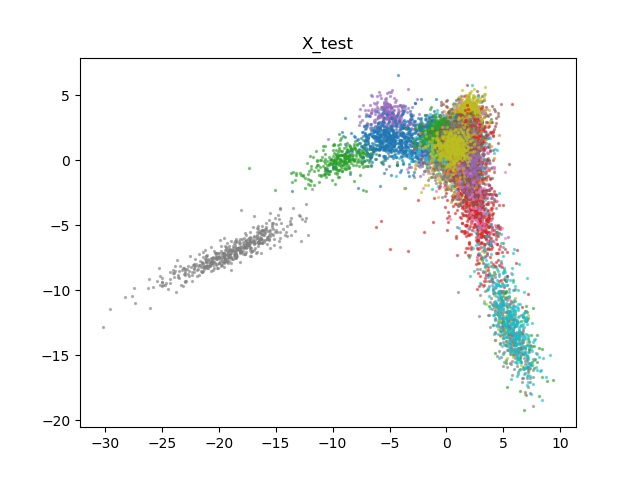
\includegraphics[width=5.5cm]{figure/X_test_scatter_2d_LDA.jpg}
}
\caption{Dataset 2-components scatter with LDA}
\label{Fig4}
\end{figure}
\end{center}

\subsubsection{AutoEncoder}
AutoEncoder is a unsupervised method to determine the essential dimensions of high-dimensional dataset, which can construct the complete dataset features with minimun loss, i.e. with encoder reducing the data dimension to `bottleneck' and decoder to restruct the data, we can get the origin sample data or get the minimun loss. In this section, we use AutoEncoder with MSE loss to get the low-dimensional feature and respectively combine linear SVM and RBF SVM to achieve the classification task. We adopt classifiction accuracy as metric in this section.

We summarize the experimental results of AutoEncoder-based model in Tab. \ref{baseline3} and Fig. \ref{Fig5}. As is shown, with the components number increases, models receive better performance especially for RBF kernel model. We can recognize that when we have less compoents, model with RBF SVM may receive a higher accuracy. AE with linear SVM and with RBF SVM respectively reach $91.42\%$ and $91.95\%$ in classification accuracy when components number comes to 1024.

We give the 2-components scattering figure of different kernel and dataset in Fig. \ref{Fig6}. We can find that some classes can't be linearly differed in 2-components, and we deem it's the reason why RBF SVM have better performance than linear one when we have less components.
\begin{center}
	\begin{figure}[htbp]
	\centering
	\subfigure[metric accuracy comparison on AutoEncoder with linear SVM]{
	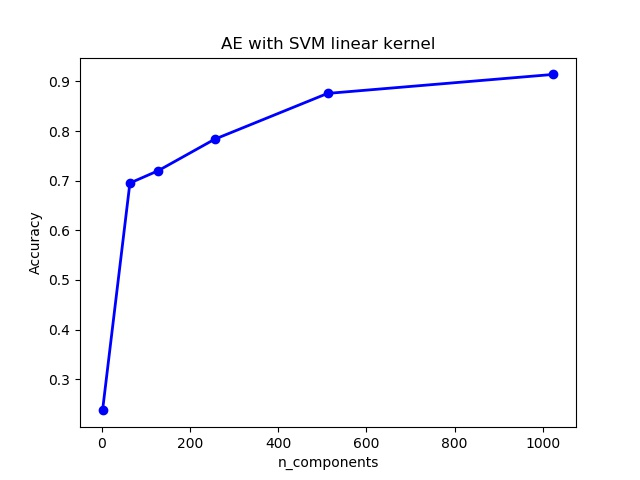
\includegraphics[width=5.5cm]{figure/AE_linear.jpg}
	%\caption{fig1}
	}
	\quad
	\subfigure[metric accuracy comparison on AutoEncoder with RBF SVM]{
	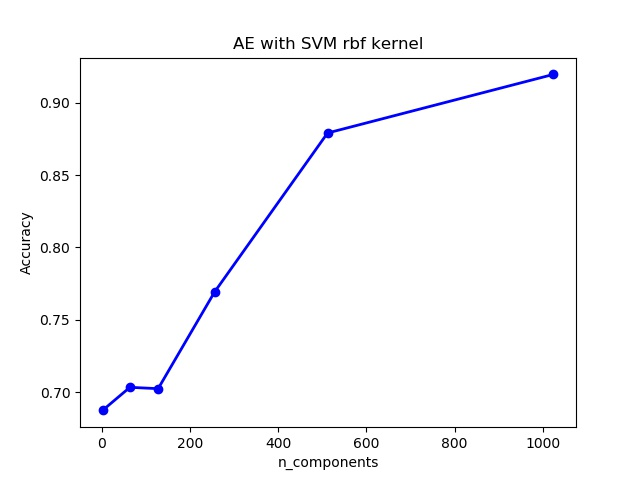
\includegraphics[width=5.5cm]{figure/AE_rbf.jpg}
	}
	\caption{AutoEncoder-based model performance on linear kernel SVM and RBF kernel SVM}
	\label{Fig5}
	\end{figure}
	\end{center}
	
	\begin{center}
	\begin{figure}[htbp]
	\centering
	\subfigure[Trainset 2D scatter with AutoEncoder]{
	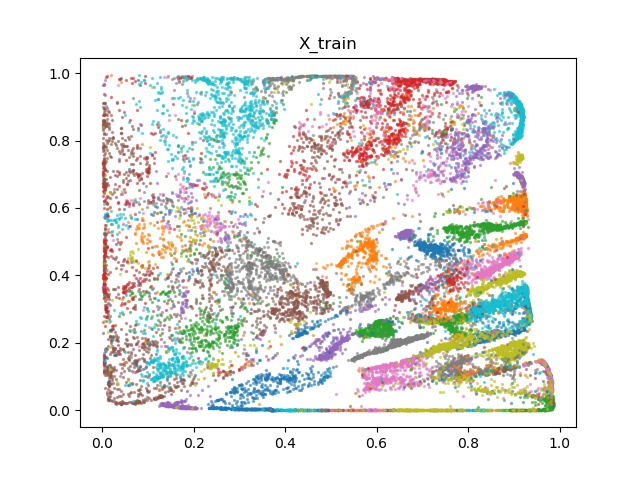
\includegraphics[width=5.5cm]{figure/X_train_scatter_2d_AE.jpg}
	%\caption{fig1}
	}
	\quad
	\subfigure[Testset 2D scatter with AutoEncoder]{
	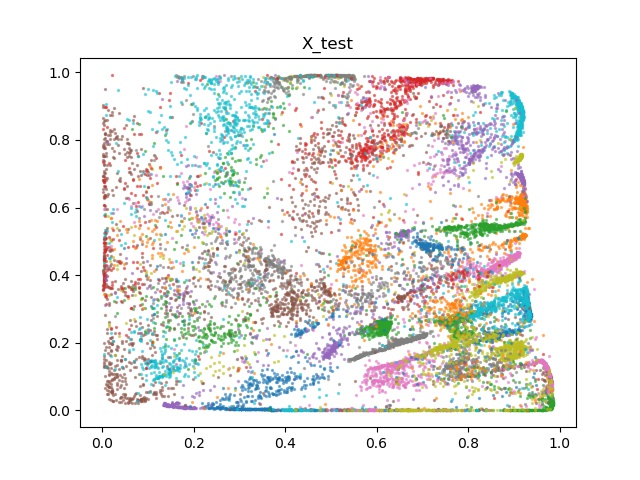
\includegraphics[width=5.5cm]{figure/X_test_scatter_2d_AE.jpg}
	}
	\caption{Dataset 2-components scatter with AutoEncoder}
	\label{Fig6}
	\end{figure}
\end{center}

\begin{table}[htbp]
	\centering
	\newcommand{\tabincell}[2]{\begin{tabular}{@{}#1@{}}#2\end{tabular}}
	\renewcommand\arraystretch{1.0}
	\caption{Comparison of AutoEncoder-based SVM and baslines in Classification Task}
	\label{baseline3}%
	\begin{tabular}{@{}p{2.5cm}<{\centering}|c|c}
		\hline
		\multirow{2}{*}{\diagbox[height=2\line,width=2.9cm,font=\tiny]{$d$}{Acc.}{$\mathit{M}$}} &\multicolumn{2}{c}{AutoEncoder+SVM}\\
		\cline{2-3}
			& {Linear kernel(\%)} & {RBF kernel(\%)}\\
		\hline
		Baseline & 93.28 & 93.52\\
		\hline
		2   & 23.71 & 68.75\\
		\hline
		64   & 69.52 & 70.35\\
		\hline
		128   & 72.01 & 70.25\\
		\hline
		256   & 78.35 & 76.93\\
		\hline
		512   & 87.59 & 87.90\\
		\hline
		1024   & \textbf{91.42} & \textbf{91.95}\\
		\hline
	\end{tabular}
\end{table}

\subsection{Feature Learning}
\subsubsection{t-SNE}

The technique t-SNE is a common method for high-dimensional data visualizing by giving each data point a location in a two or three-dimensional space. In this section, two experiment settings can derive from the rule: t-SNE used Barnes-Hut approximation to calculate gradient on dimension 2 and 3, and test parameter perplexity in $[10.0, 20.0, 30.0, 40.0, 50.0]$. 

tSNE with linear SVM receives its best performance $5.39\%$ when $perplexity=10.0$ while tSNE with RBF SVM reaches $5.95\%$ when $perplexity=10.0$. We deem the reason of low accuracy is that aim components number is not enough to extract efficient features to predict.

We also give the 2-components scattering result in Fig. \ref{Fig7}. tSNE enables different data clusters in low-dimension to be distant enough and the data points belonging to the same cluster to be close, which benefits classification. As is shown, we can differ various classes in 2D scattering. Besides, we can find with the parameter $perplexity$ increase, tSNE model can process more data.

\begin{figure}[htbp]
\centering
\subfigure[Trainset 2D scatter with tSNE (perplexity=10.0)]{
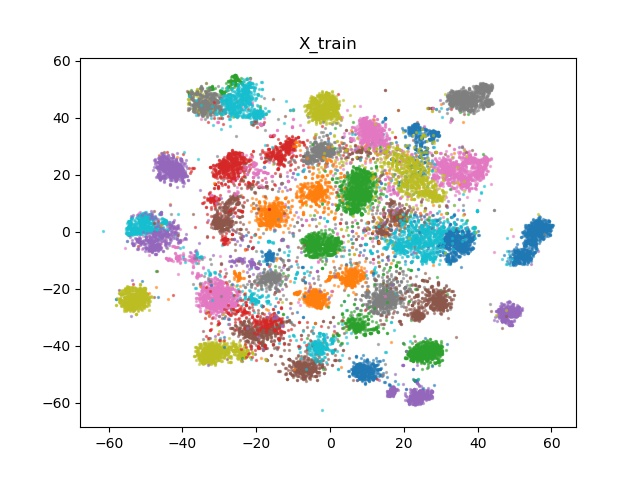
\includegraphics[width=2.5cm]{figure/X_train_scatter_2d_TSNE_10.jpg}
%\caption{fig1}
}
\quad
\subfigure[Trainset 2D scatter with tSNE (perplexity=20.0)]{
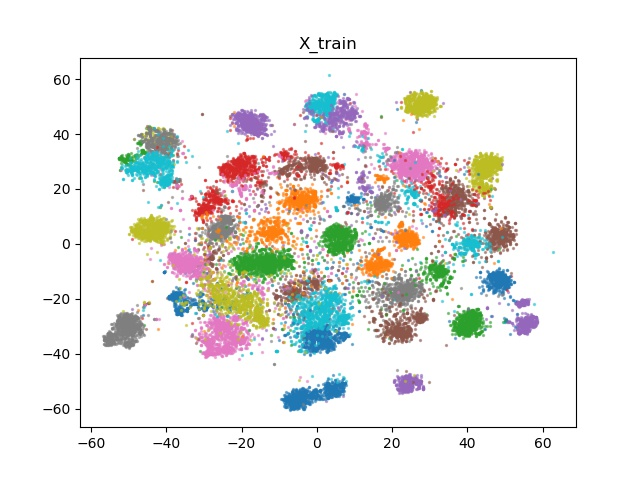
\includegraphics[width=2.5cm]{figure/X_train_scatter_2d_TSNE_20.jpg}
}
\quad
\subfigure[Trainset 2D scatter with tSNE (perplexity=30.0)]{
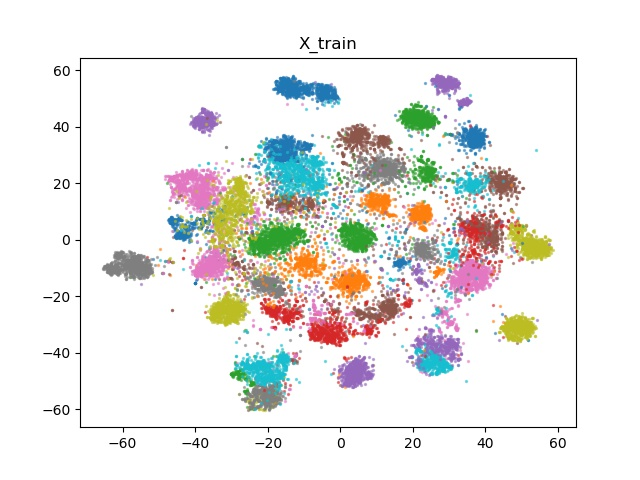
\includegraphics[width=2.5cm]{figure/X_train_scatter_2d_TSNE_30.jpg}
}
\quad
\subfigure[Trainset 2D scatter with tSNE (perplexity=40.0)]{
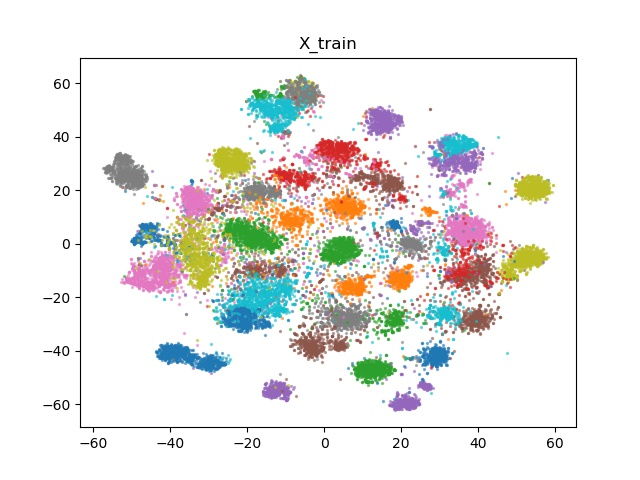
\includegraphics[width=2.5cm]{figure/X_train_scatter_2d_TSNE_40.jpg}
}
\quad
\subfigure[Trainset 2D scatter with tSNE (perplexity=50.0)]{
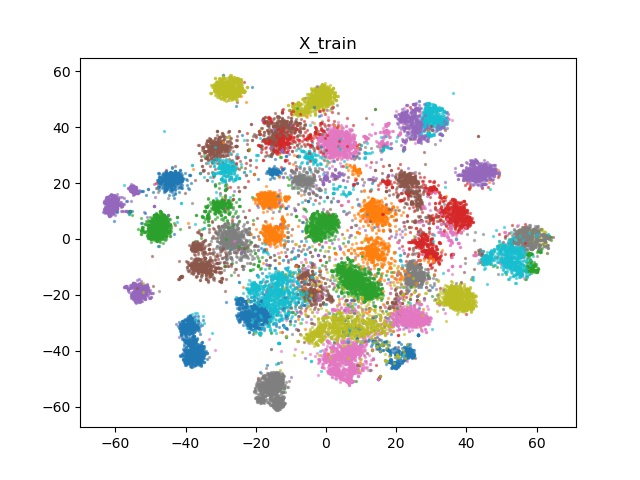
\includegraphics[width=2.5cm]{figure/X_train_scatter_2d_TSNE_50.jpg}
}
\quad
\subfigure[Testset 2D scatter with tSNE (perplexity=10.0)]{
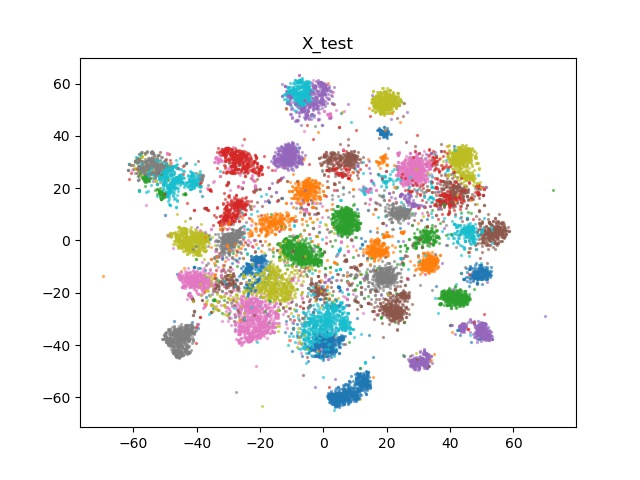
\includegraphics[width=2.5cm]{figure/X_test_scatter_2d_TSNE_10.jpg}
}
\quad
\subfigure[Trainset 2D scatter with tSNE (perplexity=20.0)]{
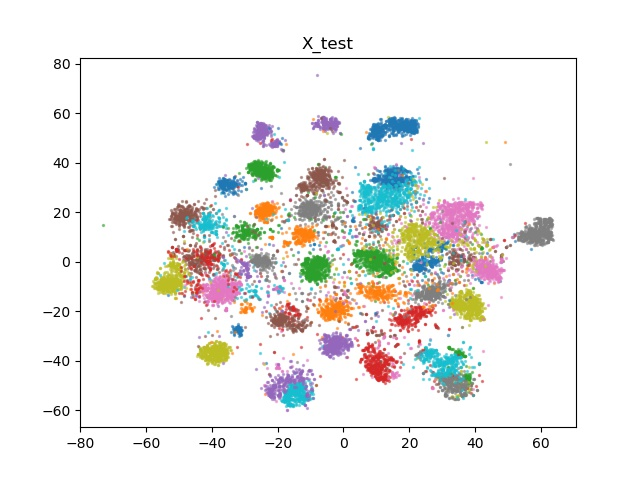
\includegraphics[width=2.5cm]{figure/X_test_scatter_2d_TSNE_20.jpg}
}
\quad
\subfigure[Testset 2D scatter with tSNE (perplexity=30.0)]{
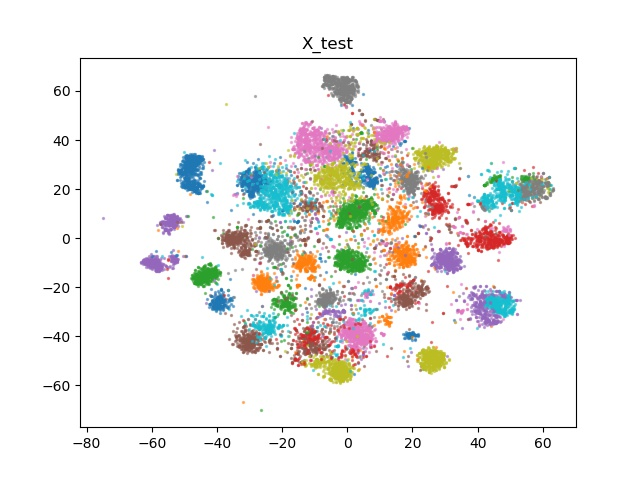
\includegraphics[width=2.5cm]{figure/X_test_scatter_2d_TSNE_30.jpg}
}
\quad
\subfigure[Trainset 2D scatter with tSNE (perplexity=40.0)]{
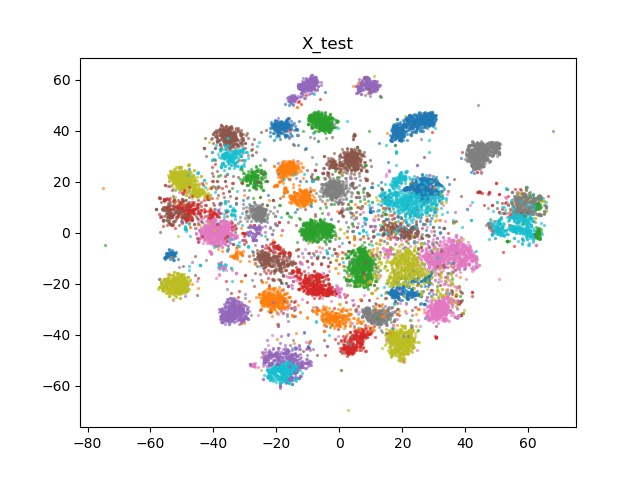
\includegraphics[width=2.5cm]{figure/X_test_scatter_2d_TSNE_40.jpg}
}
\quad
\subfigure[Testset 2D scatter with tSNE (perplexity=50.0)]{
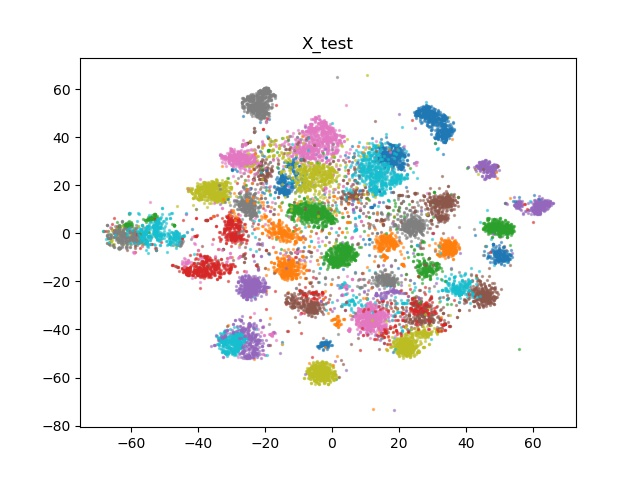
\includegraphics[width=2.5cm]{figure/X_test_scatter_2d_TSNE_50.jpg}
}
\caption{Dataset 2D scatter with tSNE on perplexity of $\{10.0,20.0,30.0,40.0,50.0\}$}
\label{Fig7}
\end{figure}

\subsubsection{LLE}
Locally Linear Embedding (LLE) is a feature learning mathod which tried to keep the linear relation between neighbor samples. In this section, we respectively use 4, 8 and 16 neighbors to rule the experiments and our aim components range is $[2, 3, 50, 100, 500, 1000, 2000]$.

We summarize the experimental results of AutoEncoder-based model in Tab. \ref{baseline3} and Fig. \ref{Fig8}. We can find if we maintain more neighbor relations and more aim components, we can get almost better performance, i.e. LLE with Linear SVM receives $90.60\%$ and LLE with RBF SVM receives $90.18\%$. Performance of LLE is satisfiying beacause original features may have simple structure and the data is randomly scatering in the high-dimension space.

We also give the 2-components scattering result in Fig. \ref{Fig9}. When we use 4 neighbors to reconstruct the sample, we can find its poor performance. For data can be regarded as manifold structure, LLE performs while when we give the proper neighbors' number.

\begin{table}[htbp]
	\centering
	\newcommand{\tabincell}[2]{\begin{tabular}{@{}#1@{}}#2\end{tabular}}
	\renewcommand\arraystretch{1.0}
	\caption{Comparison of LLE-based SVM and baslines in Classification Task}
	\label{baselin4}%
	\begin{tabular}{@{}p{2.5cm}<{\centering}|c|c|c|c|c|c}
		\hline
		\multirow{3}{*}{\diagbox[height=3\line,width=2.9cm,font=\tiny]{$\#neigh.$}{Acc.}{$\mathit{M}$}} &\multicolumn{6}{c}{LLE+SVM}\\
		\cline{2-7}
		 & \multicolumn{3}{c|}{Linear kernel(\%)} & \multicolumn{3}{c}{RBF kernel(\%)}\\
		\cline{2-7}
		 & 4 & 8 & 16 & 4 & 8 & 16\\
		\hline
		Baseline & 93.28 & 93.28 & 93.28 & 93.52 & 93.52 & 93.52\\
		\hline
		2   & 10.12 & 15.93 & 15.13 & 23.19 & 48.47 & 44.62\\
		\hline
		3   & 11.57 & 18.55 & 17.81 & 26.21 & 49.43 & 47.65\\
		\hline
		50   & 77.72 & 78.67 & 80.82 & 80.91 & 84.18 & 84.79\\
		\hline
		100   & 85.20 & 86.72 & 86.69 & 87.18 & 88.87 & 89.08\\
		\hline
		500   & 88.47 & 89.70 & 90.15 & \textbf{88.62} & \textbf{89.69} & 90.07\\
		\hline
		1000   & 88.74 & \textbf{89.93} & 90.48 & 88.49 & 89.58 & 90.12\\
		\hline
		2000   & \textbf{88.82} & 89.70 & \textbf{90.60} & 88.49 & 89.48 & \textbf{90.18}\\
		\hline
	\end{tabular}
\end{table}

\begin{center}
\begin{figure}[htbp]
\centering
\subfigure[metric accuracy comparison on LLE with linear SVM]{
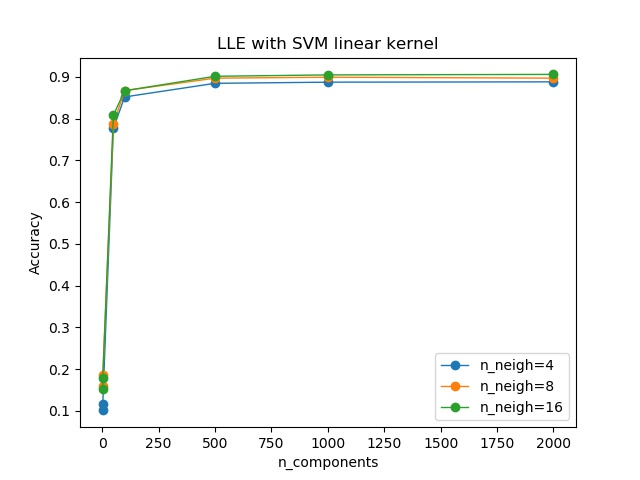
\includegraphics[width=5.5cm]{figure/LLE_linear.jpg}
%\caption{fig1}
}
\quad
\subfigure[metric accuracy comparison on LLE with RBF SVM]{
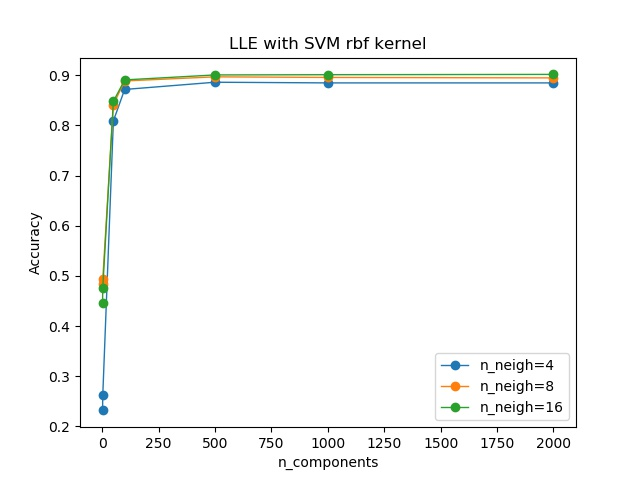
\includegraphics[width=5.5cm]{figure/LLE_rbf.jpg}
}
\caption{LLE-based model performance on linear kernel SVM and RBF kernel SVM}
\label{Fig8}
\end{figure}
\end{center}

\begin{figure}
\centering
\subfigure[Trainset 2D scatter with LLE (neighbor\_num=4)]{
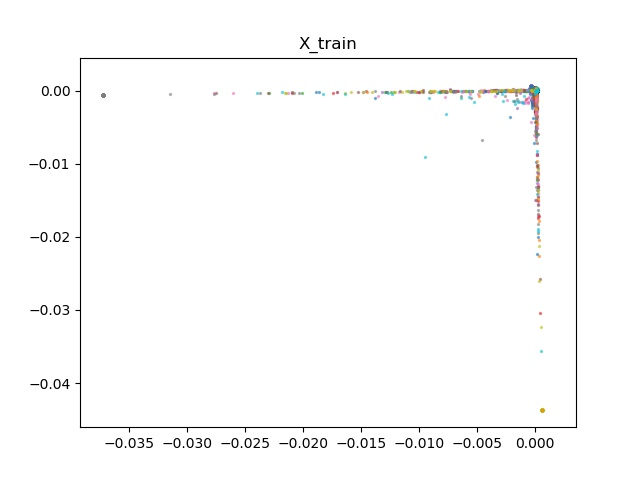
\includegraphics[width=4.1cm]{figure/X_train_scatter_2d_LLE_4.jpg}
%\caption{fig1}
}
\quad
\subfigure[Trainset 2D scatter with LLE (neighbor\_num=8)]{
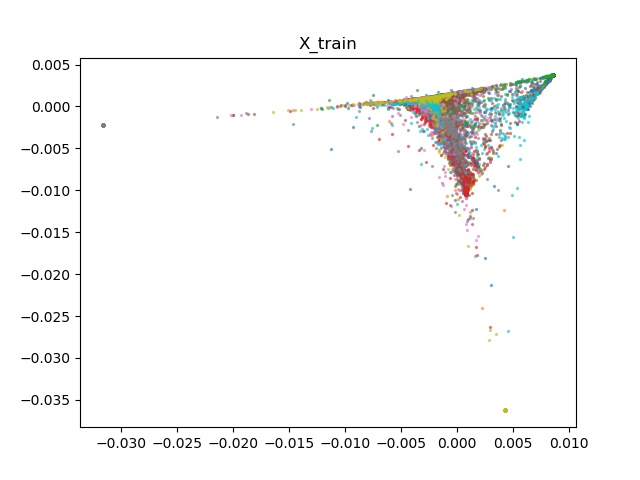
\includegraphics[width=4.1cm]{figure/X_train_scatter_2d_LLE_8.jpg}
}
\quad
\subfigure[Trainset 2D scatter with LLE (neighbor\_num=16)]{
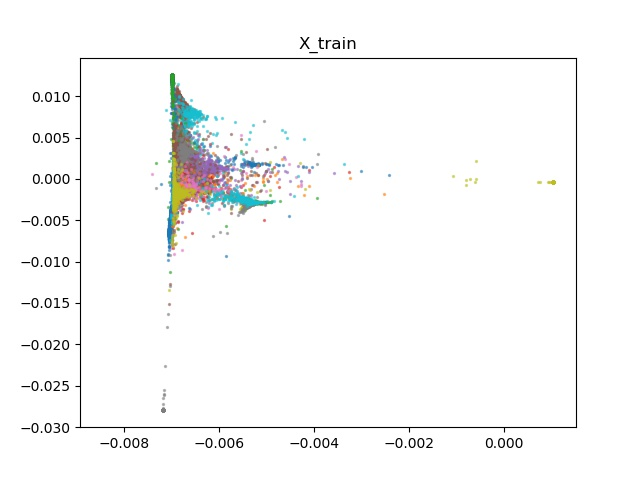
\includegraphics[width=4.1cm]{figure/X_train_scatter_2d_LLE_16.jpg}
}
\quad
\subfigure[Testset 2D scatter with LLE (neighbor\_num=4)]{
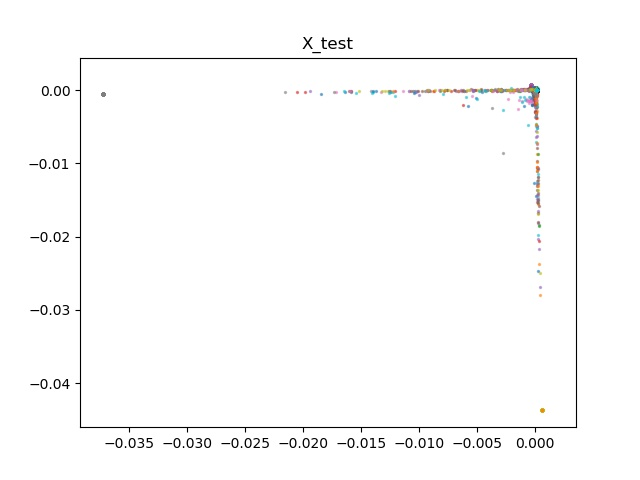
\includegraphics[width=4.1cm]{figure/X_test_scatter_2d_LLE_4.jpg}
}
\quad
\subfigure[Testset 2D scatter with LLE (neighbor\_num=8)]{
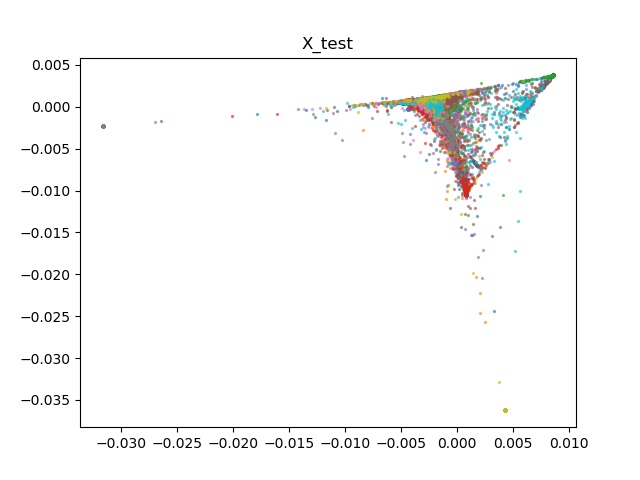
\includegraphics[width=4.1cm]{figure/X_test_scatter_2d_LLE_8.jpg}
}
\quad
\subfigure[Testset 2D scatter with LLE (neighbor\_num=16)]{
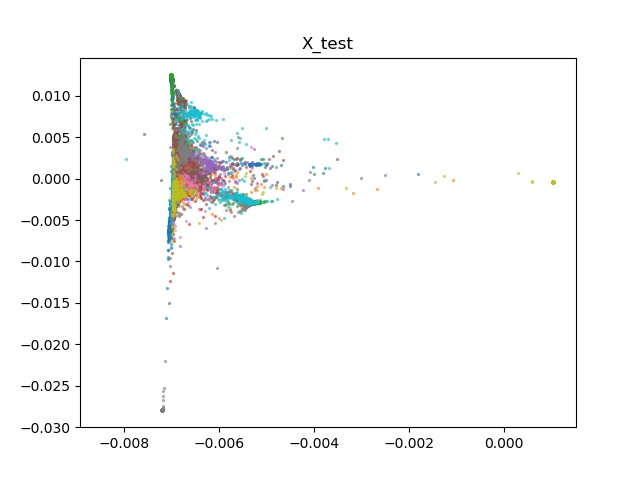
\includegraphics[width=4.1cm]{figure/X_test_scatter_2d_LLE_16.jpg}
}
\caption{Dataset 2D scatter with LLE on neighbors of $\{4, 8, 16\}$}
\label{Fig9}
\end{figure}

\section{Conclusion}
In this project, we evaluate different dimension reduction techniques by measuring their classification performance when combined with SVM model. In this Section, we want to give our perspectives on drawbacks and merits of these dimension reduction method. Importantly, we'll conclude the situations to use these methods. In general, we think feature projection and feature learning have better average performance than feature selection since minimizing effective information loss. We think kernelPCA is a universal method for dimension reduction while LDA receives a lot in the classification tasks. AutoEncoder is a good choice for generative model. In learning model, t-SNE has advantages in data visualization while LLE have great performance for data’s manifold structure.

\bibliography{bibfile.bib}
\end{document}